\vspace{\baselineskip}
\begin{figure}[h]
	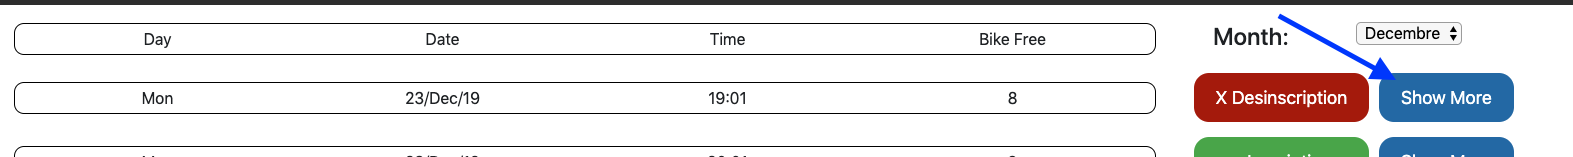
\includegraphics[width=0.9\textwidth,center]{Figures/us6-1}
	\caption{Bouton d'affichage}
\end{figure}

\begin{figure}[h]
	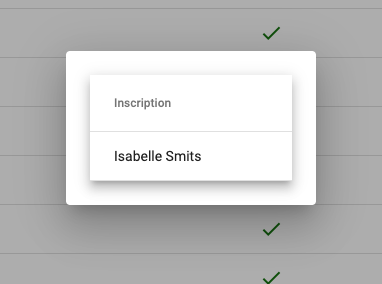
\includegraphics[width=0.5\textwidth,center]{Figures/us6-2}
	\caption{Liste Participant(e)s}
\end{figure}

\begin{enumerate}
	\item L'utilisateur trouve la session qui l'intéresse. 
	\item L'utilisateur clique sur le bouton information dans la colonne \textit{Liste Participant(e)s}. 
	\item Un tableau s'affiche avec la liste des inscrit(e)s. 
\end{enumerate}